


\section{Throughput et roulette russe}
\subsection{Le throughput}
Le throughput se définit comme suit : il représente la contribution cumulée d’un chemin indépendamment de la lumière. Exemple : un rayon qui rebondit sur un mur, puis sur le sol, avant de terminer au niveau de notre œil, va être « modifié » par le mur puis le sol avant d’arriver à l’\oe il de l’observateur. Le throughput ici va représenter le poids cumulé causé par les interactions avec les objets.\\
$$inserer\ schema\ throughput$$
Ainsi, le throughput $T$ sera calculer de la manière suivante:

Pour un chemin excluant la source de lumière, composé de $N$ primitives:

$$T=\Pi^N_{i=1}T_i\text{	,   avec }T_i=albedo_i$$
la contribution d'un chemin s'écrit donc:
$$
C=L_e(x_d)\cdot T
$$

Comme les matériaux que nous utilisons sont tous lambertiens, le throughput sera toujours le produit de l'albédo de chaque primitive intersectée par le rayon.
\subsection{Roulette russe}
\subsubsection{État de l'art}
La roulette russe est une technique issue du transport de particules en physique nucléaire, où elle est utilisée depuis les années 1940 pour simuler le parcours des neutrons dans la matière\footnote{Arvo J., Kirk D., Particle Transport and Image Synthesis, SIGGRAPH 1990}.\\
 
Appliquée à Monte Carlo, cela se traduit comme suit : maintenant que nous avons une donnée quantifiable sur la contribution d’un chemin, on peut décider de stopper les chemins qui contribuent très peu (donc avec un throughput faible). Cependant, simplement supprimer ces chemins introduit un biais en favorisant ceux qui contribuent beaucoup et, de ce fait, provoque une perte d’énergie lumineuse.\\

\subsubsection{Implémentation}

Pour éviter ce biais, nous choisissons de couper un chemin selon cette condition :
\begin{itemize}
	\item[$\bullet$] Nous tirons un nombre aléatoire $\epsilon$
	\item[$\bullet$] Si $\epsilon$ est supérieur à la composante maximale du throughput (notée p), nous stoppons le chemin
	\item[$\bullet$] Si le chemin survit, nous divisons le throughput par p
\end{itemize}


\section{Accélération par arbre BVH}
\subsection{Etat de l'art}
La hiérarchie de volumes englobants (Bounding Volume Hierarchy, BVH) est devenue la structure d'accélération dominante pour le lancer de rayons depuis les années 2000. En effet, elle organise les primitives d'une scène dans un arbre binaire dont chaque n\oe ud stocke une AABB englobant celles de ses descendants\footnote{Rubin S. M., Whitted T., A 3-Dimensional Representation for Fast Rendering of Complex Scenes, SIGGRAPH 1980.
}\footnote{Kay T. L., Kajiya J. T., Ray Tracing Complex Scenes, SIGGRAPH 1986.}.\\
Ainsi, la construction de l'arbre se fera avec la méthode des centroïdes. Nous allons appeler "centroïdes d'une primitive" le centre de l'AABB la plus petite contenant la primitive. Cette méthode se fait comme suit: à chaque n\oe ud, nous calculons l'AABB des centroïdes des primitives, on choisit comme axe de coupe son axe le plus long, puis on partitionne par médiane. La récursion s'arrête lorsqu'un n\oe ud contient moins de 1 et 4 pour un compromis raisonnable entre profondeur d'arbre et coût des feuilles. La traversée est en O($\log$ n) en moyenne.\\
Cette approche à l'avantage de pouvoir sauter des branches entières en fonction de la position de l'AABB englobante du n\oe ud. Exemple: une AABB derrière un rayon ne sera jamais intersectée par ce dernier, il va donc ignorer tous les objets se trouvant à l'intérieur.
\subsection{Implémentation}

\subsubsection{Construction de l'arbre}

Jusqu'ici, nous travaillons sur un tableau de structures de primitives. Notre objectif va être de repartir ces primitives dans un arbre BVH décrit dans l'algorithme 1.

\begin{algorithm}
\caption{Construction récursive de l'arbre BVH}
\begin{algorithmic}
\Require Un nœud $n$, un tableau de primitives $P$ de taille $N$, une profondeur $d$
\Ensure Un arbre BVH dont la racine est $n$

\State Calculer l'AABB englobante de toutes les primitives de $P$, affecter à $n.\text{box}$

\If{$N \leq $ \texttt{MAX\_OBJECTS}}
    \State Stocker toutes les primitives de $P$ dans $n.\text{objects}$ \Comment{nœud feuille}
    \State \Return
\EndIf

\State Calculer les dimensions de $n.\text{box}$ sur les axes $x$, $y$, $z$
\State $\text{axis} \leftarrow$ l'axe de dimension maximale

\State Trier $P$ par coordonnée du centroïde de l'AABB de chaque primitive selon $\text{axis}$
\State $\text{split} \leftarrow$ coordonnée du centroïde médian

\State Partitionner $P$ en $P_L$ (centroïde $<$ split) et $P_R$ (centroïde $\geq$ split)

\If{$\min(|P_L|, |P_R|) / N < 0.2$ \textbf{ou} $\max(|P_L|, |P_R|) / N > 0.9$}
    \State $P_L \leftarrow P[0\,\ldots\,\lfloor N/2 \rfloor - 1]$,\quad $P_R \leftarrow P[\lfloor N/2 \rfloor\,\ldots\,N-1]$
    \Comment{partitionnement forcé par médiane}
\EndIf

\State Créer les enfants $n.\text{left}$ et $n.\text{right}$
\State \Call{ConstructionBVH}{$n.\text{left},\; P_L,\; |P_L|,\; d+1$}
\State \Call{ConstructionBVH}{$n.\text{right},\; P_R,\; |P_R|,\; d+1$}
\State Mettre à jour $n.\text{box}$ depuis les AABB des deux enfants
\end{algorithmic}
\end{algorithm}


Cette construction se fait en O(N$\cdot$ $\log$ N), contrairement à celle du tableau en O(1). Cette différence aura un impact important pour un grand nombre de primitives. Cependant, cette perte de performance sera compensée par le parcours de l'arbre en O($\log$ N) pour les intersection à la place de celle en O(N) pour l'approche naïve. De plus, le temps de l'initialisation de l'arbre est bien négligeable par rapport à celui du rendu de l'image, ce qui compense largement la construction de l'arbre.


\subsubsection{Parcours de l'arbre durant pour l'intersection la plus proche}

Le rayon est envoyé dans une direction $\vec{d}$ d'une origine $O$. Pour déterminer l'intersection, nous allons calculer le plus petit réel positif $t_{AABB}$ tel que: $I=O+t_{AABB}\cdot \vec d$ avec l'AABB de la racine de l'arbre. S'il n'existe pas, cela veut dire que le rayon n'intersecte pas l'AABB, et donc aucune primitive de l'espace. S'il existe, nous ferons de-même pour les 2 enfants de la racine, et ainsi de suite. Lorsque le rayon intersecte une feuille, nous calculerons le $t$ pour chaque primitive dans la feuille.\\

L'algorithme s'arrêtera lorsque le rayon aura vérifier l'intersection pour chaque n\oe ud. Le point d'intersection sera donc le $t$ positif le plus petit.\\

\begin{algorithm}
\caption{Intersection d'un rayon avec l'arbre BVH}
\begin{algorithmic}
\Require Un nœud $n$, un rayon $r$, le $t$ courant le plus proche $t_{\min}$
\Ensure La primitive intersectée la plus proche et son $t$, ou aucune intersection

\If{\Call{IntersectionAABB}{$r,\; n.\text{box}$} $< 0$}
    \State \Return \textbf{aucune intersection}
\EndIf

\If{$n$ est une feuille}
    \For{chaque primitive $p \in n.\text{objects}$}
        \State $t \leftarrow$ \Call{IntersectionPrimitive}{$r,\; p$}
        \If{$t > \varepsilon$ \textbf{et} $t < t_{\min}$}
            \State $t_{\min} \leftarrow t$,\quad primitive intersectée $\leftarrow p$
        \EndIf
    \EndFor
    \State \Return
\EndIf

\State $t_L \leftarrow$ \Call{IntersectionAABB}{$r,\; n.\text{left}.\text{box}$}
\State $t_R \leftarrow$ \Call{IntersectionAABB}{$r,\; n.\text{right}.\text{box}$}

\State $(\text{premier}, \text{second}) \leftarrow$ ordonner les enfants par $t$ croissant

\If{$t_{\text{premier}} \geq 0$}
    \State \Call{IntersectionBVH}{$\text{premier},\; r,\; t_{\min}$}
\EndIf
\If{$t_{\text{second}} \geq 0$}
    \State \Call{IntersectionBVH}{$\text{second},\; r,\; t_{\min}$}
\EndIf
\end{algorithmic}
\end{algorithm}

\subsection{limites}

Cet algorithme possède des limites. En effet,  la partition par médiane sur un seul axe peut produire des AABB qui se chevauchent fortement quand les objets sont distribués irrégulièrement. \\
Pour palier à ce problème, une solution réside dans le clustering. Pour la suite, nous ferons un clustering par la méthode des K-moyennes.

\section{Accélération par clustering des K-moyennes}

\subsection{État de l'art}

Le K-means est l'une des méthodes de partitionnement non supervisé les plus anciennes et les plus utilisées. L'objectif du K-means est de partitionner P en $k$ clusters disjoints $\left(C_1,..., C_k\right)$, avec $k$ fixé à l'avance $\left(k \ll N\right)$, tels que chaque point soit affecté à exactement un cluster. Chaque cluster $C_j$ est représenté par son centroïde $\mu_j \in\ \mathbb{R}^3$.\\
On cherchera ensuite à résoudre la fonction objective suivante:
$$\min\left\{ J(C_1,..., C_k, \mu_1,..., \mu_k) \right\}\text{tel que: }J=\sum_{j=1}^k\sum_{p \in C_j}\left|\left|p-\mu_j\right|\right|^2\atop
\text{avec $p$, un centroïde de primitive}$$

L'un des premier algorithme à résoudre cette fonction objective est l'algorithme de Lloyd\footnote{Lloyd S. P., Least Squares Quantization in PCM, IEEE Trans. Information Theory, 1982}, que nous utiliserons dans la suite de ce projet.

\subsection{Implémentation de l'arbre BVH par les K-moyennes}

\subsubsection{Détermination des clusters}
Dans un premier temps, nous utiliserons l'algorithme de Lloyd suivant: pour une itération $i$, on associe chaque centroïde de primitive $p$ au point $\mu_j$ le plus proche, déterminée par la norme euclidienne $\left|\left|p-\mu_j\right|\right|^2$. Ensuite, nous recalculons les centres des clusters $C_j$, $\mu_j$, comme étant la moyenne de la position de chaque point $p$ associé.\\

\begin{algorithm}
\caption{Construction de l'arbre BVH par K-moyennes}
\begin{algorithmic}
\Require Un ensemble de $N$ primitives $\mathcal{P}$, un entier $K$, \texttt{MAX\_ITER} itérations
\Ensure $K$ clusters, chacun associé à un arbre BVH local

\State Calculer le centroïde $c_i$ de l'AABB de chaque primitive $p_i \in \mathcal{P}$

\State Initialiser les $K$ centres $\{\mu_k\}_{1 \leq k \leq K}$ en tirant $K$ centroïdes distincts aléatoirement dans $\{c_i\}$

\For{$\text{iter} = 1$ \textbf{à} \texttt{MAX\_ITER}}
    \For{chaque primitive $p_i$}
        \State $k^* \leftarrow \arg\min_k \|c_i - \mu_k\|^2$
        \State Affecter $p_i$ au cluster $C_{k^*}$
    \EndFor
    \For{chaque cluster $C_k$}
        \If{$|C_k| > 0$}
            \State $\mu_k \leftarrow \dfrac{1}{|C_k|}\displaystyle\sum_{p_i \in C_k} c_i$
        \Else
            \State $\mu_k \leftarrow$ centroïde aléatoire parmi $\{c_i\}$
        \EndIf
    \EndFor
\EndFor

\For{chaque cluster $C_k$}
    \State Calculer l'AABB englobante de $C_k$
    \State \Call{ConstructionBVH}{racine$_k$, $C_k$, $|C_k|$, $0$}
\EndFor
\State Calculer l'AABB globale englobant les $K$ AABB de clusters
\end{algorithmic}
\end{algorithm}

Les points $\mu_j$ seront initialisés aléatoirement parmi l'ensemble $P=\left\{p_i\right\}_{0 \leq i \leq N}$.\\

Ces $k$ clusters, composé chacun d'un tableau de primitives, seront les points de départ pour former k arbres BVH, décrits précédemment.\\

Ainsi, nous utiliserons la même méthode pour déterminer les intersections des rayons sur les primitives décrite précédemment, pour chaque BVH construit de cette manière.\\

Le K-means résout le problème de chevauchement des AABB de l'arbre BVH classique en groupant d'abord les objets spatialement proches avant de construire les BVH locaux.


\section{SIMD du path tracer naïf}

\subsection{Introduction}

Dans cette partie, nous allons détailler une implémentation SIMD à la main afin d'identifier d'éventuels gains de performance.

\subsubsection{Vectorisation}

Les architectures CPU modernes (x86 ou ARM) permettent deux types d'opérations :
les opérations scalaires et les opérations vectorielles.

Code C :

\begin{lstlisting}[language=C]
float a = 2;
float b = 3;
float c = a + b;
\end{lstlisting}

Code assembleur :

\begin{lstlisting}
movss xmm0, DWORD PTR .LC0[rip]
movss DWORD PTR [rbp-4], xmm0
\end{lstlisting}

Code C :

\begin{lstlisting}[language=C]
for (int i = 0; i < N; ++i)
    c[i] = a[i] + b[i];
\end{lstlisting}

Code assembleur :

\begin{lstlisting}
.L7:
    movaps xmm0, XMMWORD PTR [rcx+rax]
    addps xmm0, XMMWORD PTR [rdx+rax]
\end{lstlisting}

\subsubsection{Vectorisation manuelle}

Il arrive parfois que le compilateur ne puisse pas vectoriser automatiquement certaines boucles. Dans ce cas, on peut utiliser des intrinsics pour forcer une vectorisation.

Code C :

\begin{lstlisting}[language=C]
# N divisible par 4
for (int i = 0; i < N; i += 4)
{
    __m128 a_vec = _mm_load_ps(a + i);
    __m128 b_vec = _mm_load_ps(b + i);
    __m128 c_vec = _mm_add_ps(a_vec, b_vec);

    _mm_store_ps(c + i, c_vec);
}
\end{lstlisting}

Code assembleur :

\begin{lstlisting}
.L4:
    vaddps xmm0, xmm0, XMMWORD PTR [rbp-1040+rax]
    vmovaps XMMWORD PTR [rbp-528+rax], xmm0
\end{lstlisting}

\FloatBarrier

\subsection{Structure de données}

Notre code de base suit le modèle *Array of Structures* (AoS). Ce modèle peut dégrader la localité des données dans le cache.
Pour améliorer la localité mémoire et la vectorisation, on utilise une structure de type *Structure of Arrays* (SoA).

\begin{lstlisting}[language=C]
typedef struct fSphere
{
    __attribute__((aligned(16))) float *coord;
    __attribute__((aligned(16))) float *x;
    __attribute__((aligned(16))) float *y;
    __attribute__((aligned(16))) float *z;
    __attribute__((aligned(16))) float *albedo;
    __attribute__((aligned(16))) float *r;
    __attribute__((aligned(16))) float *g;
    __attribute__((aligned(16))) float *b;
    __attribute__((aligned(16))) float *radius;
    __attribute__((aligned(16))) float *type;
    __attribute__((aligned(16))) float *emission_power;

    uint64_t size;
    uint64_t capacity;
    uint64_t padding;
    uint64_t chunked_size;

} fSphere;
\end{lstlisting}

\subsection{Alignement mémoire}

\lstinline|__attribute__((aligned(16)))| indique un alignement mémoire sur 16 octets, nécessaire pour certaines instructions SIMD (SSE).

Cependant, cela n'implique pas que tous les éléments d'un tableau soient alignés individuellement. Pour cela, on utilise une allocation alignée :

\begin{lstlisting}[language=C]
void *aligned_alloc(size_t alignment, size_t size);
\end{lstlisting}
On arrondie par un entier multiple de 4 pour éviter des tail loop.

\href{https://en.cppreference.com/w/c/memory/aligned_alloc}{aligned\_alloc (cppreference)}

\FloatBarrier

\subsection{Rayons}

Le path tracing fonctionne de la manière suivante :

\begin{enumerate}
\item Un rayon est lancé depuis la caméra
\item Si le rayon touche une surface, on échantillonne la couleur selon le matériau
\item Le rayon est rebondi jusqu'à une source lumineuse ou un nombre maximal de rebonds
\end{enumerate}

\begin{figure}[H]
\centering
\begin{tikzpicture}[>=Stealth]

\node (cam) at (0,0) {Caméra};

\coordinate (surface_0) at (2,1);
\coordinate (surface_1) at (2,-1);

\draw[gray] (1,1) -- (3,1);
\draw[gray] (1,-1) -- (3,-1);

\node[circle, fill=yellow, minimum size=0.8cm] (light) at (6,3) {Lumière};

\draw[->, thick] (cam) -- (surface_0);
\draw[->, thick, red] (surface_0) -- (surface_1);
\draw[->, thick, blue] (surface_1) -- (light);

\end{tikzpicture}
\caption{Path tracing avec rebonds de rayons}
\end{figure}

Avec SIMD, on traite plusieurs rayons simultanément.

\begin{enumerate}
\item Quatre rayons sont lancés depuis la caméra
\item Les intersections sont calculées en parallèle
\item Les rayons sont rebondis simultanément
\end{enumerate}

\begin{figure}[H]
\centering
\begin{tikzpicture}[>=Stealth]

\node (cam) at (0,0) {Caméra};

\coordinate (s0) at (2,1);
\coordinate (s1) at (2,-1);
\coordinate (s2) at (5,1);
\coordinate (s3) at (5,-1);

\draw[gray] (1,1) -- (3,1);
\draw[gray] (1,-1) -- (3,-1);
\draw[gray] (4,1) -- (6,1);
\draw[gray] (4,-1) -- (6,-1);

\node[circle, fill=yellow, minimum size=0.8cm] (light) at (8,0) {Lumière};

\draw[->, thick, red] (cam) -- (s0);
\draw[->, thick, red] (cam) -- (s1);
\draw[->, thick, red] (cam) -- (s2);
\draw[->, thick, red] (cam) -- (s3);

\draw[->, thick, blue] (s0) -- (light);
\draw[->, thick, blue] (s1) -- (light);
\draw[->, thick, blue] (s2) -- (light);
\draw[->, thick, blue] (s3) -- (light);

\end{tikzpicture}
\caption{SIMD path tracing avec 4 rayons traités en parallèle}
\end{figure}

\FloatBarrier

Ainsi, la structure d'un rayon ressemble à ça :

\begin{lstlisting}[language=C]
typedef struct vRay
{
    __vec4f ori_x;
    __vec4f ori_y;
    __vec4f ori_z;

    __vec4f dir_x;
    __vec4f dir_y;
    __vec4f dir_z;

} vRay;
\end{lstlisting}

\subsection{Intersections}

Le principe du path tracing repose sur la simulation du trajet de la lumière dans une scène 3D. À chaque rebond, il est nécessaire de déterminer si un rayon intersecte une ou plusieurs primitives géométriques, et d'en déduire le point d'impact le plus proche.

Cette étape d'intersection constitue l'un des principaux goulots d'étranglement du rendu, car elle est exécutée un très grand nombre de fois : chaque pixel génère plusieurs rayons, et chaque rayon peut potentiellement être testé contre l'ensemble des objets de la scène.

Dans une implémentation naïve, le coût est donc proportionnel à :
\[
O(N_{rays} \times N_{objects})
\]

L'objectif de cette section est de présenter une implémentation SIMD de la fonction d'intersection afin de réduire le nombre d'instructions nécessaires par calcul.

L'implémentation SIMD présentée ici repose sur une vectorisation des rayons : quatre rayons sont traités simultanément, tandis que les primitives sont parcourues séquentiellement.

Cette approche permet de conserver une structure simple tout en exploitant efficacement les unités vectorielles du processeur.
\begin{lstlisting}[language=C]

bool intersect_sphere(Ray* const r, Vector *center, float radius, Vector *hit)
{
	Vector oc;
	sub_ext(&r->position, center, &oc);
	

	const float A = dot(&r->direction, &r->direction);
	const float B = 2.0f * dot(&r->direction, &oc);
	const float C = dot(&oc, &oc) - radius * radius;

	const float delta = B*B - 4.0f*A*C;

	if (delta < 0.0f)
		return false;

	float sqrt_delta = sqrtf(delta);
	float t0 = (-B - sqrt_delta) / (2.0f * A);
	float t1 = (-B + sqrt_delta) / (2.0f * A);

	float t = -1.0f;

	if (t0 > EPS)
		t = t0;
	else if (t1 > EPS)
		t = t1;
	else
		return false; # return false if each intersection point is negative

	linear_ext(&r->position, &r->direction, t, hit);
	return true;
}
\end{lstlisting}

\begin{figure}[H]
\centering
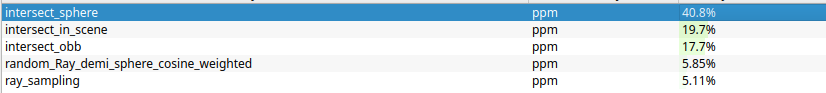
\includegraphics[scale=0.5]{include/img55}
\caption{Points chauds du code}
\end{figure}


\textbf{Principe général :} 

L'objectif est de vectoriser le calcul d'intersection en traitant quatre rayons simultanément. Contrairement à la version scalaire où un rayon est testé contre toutes les sphères, ici chaque opération SIMD manipule quatre valeurs en parallèle.

\medskip

\textbf{Étape 1 : initialisation}

\begin{lstlisting}[language=C]
__vec4f center_x_min = max_limit;
__vec4f center_y_min = max_limit;
__vec4f center_z_min = max_limit;
\end{lstlisting}

On initialise ici les positions des centres correspondant aux intersections les plus proches.  
Dans la version scalaire, on cherche la sphère la plus proche pour un rayon.  
Dans la version SIMD, on effectue cette opération pour quatre rayons simultanément.

\medskip

\textbf{Étape 2 : calcul du vecteur origine-centre}

\begin{lstlisting}[language=C]
const __vec4f center_x = set1(sph->x[i]);
const __vec4f center_y = set1(sph->y[i]);
const __vec4f center_z = set1(sph->z[i]);

const __vec4f oc_x = sub_(&packed_ray->ori_x, &center_x);
const __vec4f oc_y = sub_(&packed_ray->ori_y, &center_y);
const __vec4f oc_z = sub_(&packed_ray->ori_z, &center_z);
\end{lstlisting}

On charge le centre d'une sphère dans les quatre lanes SIMD, puis on calcule le vecteur $\vec{OC}$ entre l'origine des rayons et ce centre.

\medskip

\textbf{Étape 3 : produit scalaire}

\begin{lstlisting}[language=C]
const __vec4f h = dot_(&packed_ray->dir_x, &packed_ray->dir_y, &packed_ray->dir_z,
                       &oc_x, &oc_y, &oc_z);
\end{lstlisting}

On calcule le produit scalaire entre la direction des rayons et le vecteur $\vec{OC}$.  
Cette valeur est utilisée dans le calcul du discriminant.

\medskip

\textbf{Étape 4 : discriminant}

\begin{lstlisting}[language=C]
const __vec4f ac = mul_(&a, &c);
const __vec4f delta = fmsub(&h, &h, &ac);
const __vec4f mask_delta = greater(&delta, &epsilon);
\end{lstlisting}

Le discriminant $\Delta = h^2 - a \cdot c$ permet de déterminer si une intersection existe.  
Si $\Delta < 0$, le rayon ne touche pas la sphère.

\medskip

\textbf{Étape 5 : test rapide}

\begin{lstlisting}[language=C]
if (fuse(&mask_delta) == 0)
    continue;
\end{lstlisting}

Si aucun des quatre rayons n'intersecte la sphère, on passe directement à la suivante.

\medskip

\textbf{Étape 6 : calcul des solutions}

\begin{lstlisting}[language=C]
const __vec4f fake_delta = max_(&delta, &zero);
const __vec4f sqrt_delta = sqrt_(&fake_delta);

const __vec4f minus_h = sub_(&zero, &h);
const __vec4f t1 = mul_(&sub_(&minus_h, &sqrt_delta), &over_a);
const __vec4f t2 = mul_(&add_(&minus_h, &sqrt_delta), &over_a);
\end{lstlisting}

On calcule ici les deux solutions de l'équation quadratique correspondant aux points d'intersection.

\medskip

\textbf{Étape 7 : sélection des intersections valides}

\begin{lstlisting}[language=C]
const __vec4f test0 = greater(&t1, &epsilon);
const __vec4f test1 = greater(&t2, &epsilon);

__vec4f ts = blendv(&max_limit, &t2, &test1);
ts = blendv(&ts, &t1, &test0);
ts = blendv(&max_limit, &ts, &mask_delta);
\end{lstlisting}

On filtre les solutions négatives et on sélectionne la plus proche intersection valide.

\medskip

\textbf{Étape 8 : mise à jour du hit}

\begin{lstlisting}[language=C]
const __vec4f mask0 = lower(&ts, tmin);

if (fuse(&mask0) == 0)
    continue;

*tmin = min_(&ts, tmin);
\end{lstlisting}

On conserve uniquement les intersections les plus proches.

\medskip

\textbf{Étape 9 : calcul du point d'impact et des normales}

\begin{lstlisting}[language=C]
const __vec4f hit_point_x = fmadd(&packed_ray->dir_x, tmin, &packed_ray->ori_x);
const __vec4f hit_point_y = fmadd(&packed_ray->dir_y, tmin, &packed_ray->ori_y);
const __vec4f hit_point_z = fmadd(&packed_ray->dir_z, tmin, &packed_ray->ori_z);
\end{lstlisting}

On calcule la position du point d'impact pour chaque rayon.

\medskip

\textbf{Étape 10 : récupération des attributs}

Les normales, couleurs et propriétés des matériaux sont ensuite mises à jour à l'aide de masques SIMD afin de ne modifier que les rayons ayant réellement intersecté la sphère.

\medskip

\subsection{Échantillonnage du rayon}

\textbf{Principe général :}

L'échantillonnage des rayons permet de simuler les rebonds de la lumière sur les surfaces.  
Dans le cas d'un matériau diffus (Lambertien), les directions sont tirées aléatoirement dans une demi-sphère orientée selon la normale.

L'implémentation SIMD permet ici de générer quatre directions aléatoires simultanément.

\medskip

\textbf{Étape 1 : génération des variables aléatoires}

\begin{lstlisting}[language=C]
const float u01 = (float)rand_r(seed) / (float)RAND_MAX;
...
const float u32 = (float)rand_r(seed) / (float)RAND_MAX;

__vec4f u_n1 = set(u31, u21, u11, u01);
__vec4f u_n2 = set(u32, u22, u12, u02);
\end{lstlisting}

On génère des variables aléatoires scalaires, puis on les regroupe dans des vecteurs SIMD afin de traiter quatre échantillons en parallèle.

\medskip

\textbf{Étape 2 : conversion en coordonnées sphériques}

\begin{lstlisting}[language=C]
__vec4f atheta = sqrt_(&u_n1);
__vec4f phi = mul_(&two_pi, &u_n2);
\end{lstlisting}

On transforme les variables aléatoires en coordonnées sphériques adaptées à un échantillonnage cosinus.

\medskip

\textbf{Étape 3 : coordonnées locales}

\begin{lstlisting}[language=C]
__vec4f x = cos_(&phi);
__vec4f y = sin_(&phi);

x = mul_(&x, &atheta);
y = mul_(&y, &atheta);

__vec4f z = sub_(&one, &u_n1);
z = sqrt_(&z);
\end{lstlisting}

On obtient une direction dans une base locale où l'axe $z$ correspond à la normale.

\medskip

\textbf{Étape 4 : construction d'une base orthonormée}

\begin{lstlisting}[language=C]
__vec4f basic_x = set1(0);
__vec4f basic_y = set1(1);
__vec4f basic_z = set1(0);

__vec4f right_x = set1(1);
__vec4f right_y = set1(0);
__vec4f right_z = set1(0);
\end{lstlisting}

On définit des vecteurs permettant de construire une base locale autour de la normale.
\href{https://www.opengl-tutorial.org/fr/intermediate-tutorials/tutorial-13-normal-mapping/}{aligned\_alloc (opengl-tutorial)}

\medskip

\textbf{Étape 5 : calcul des vecteurs tangent et bitangent}

\begin{lstlisting}[language=C]
cross_(normal_x, normal_y, normal_z, &up_x, &up_y, &up_z,
       &tangent_x, &tangent_y, &tangent_z);

norm_(&tangent_x, &tangent_y, &tangent_z,
      &tangent_x, &tangent_y, &tangent_z);

cross_(&tangent_x, &tangent_y, &tangent_z,
       normal_x, normal_y, normal_z,
       &bitangent_x, &bitangent_y, &bitangent_z);
\end{lstlisting}

On construit une base orthonormée $(tangent, bitangent, normal)$.

\medskip

\textbf{Étape 6 : transformation vers l'espace monde}

\begin{lstlisting}[language=C]
tangent_x = mul_(&tangent_x, &x);
bitangent_x = mul_(&bitangent_x, &y);
__vec4f norm_x = mul_(normal_x, &z);

*dir_x = add_(&tangent_x, &bitangent_x);
*dir_x = add_(dir_x, &norm_x);
\end{lstlisting}

On combine les trois composantes pour obtenir la direction finale du rayon dans l'espace.

\medskip


\textbf{Lancer de rayons (path tracing SIMD)}

\medskip

\textbf{Principe général :}

Cette fonction simule les rebonds successifs d'un paquet de quatre rayons dans la scène.  
Chaque rayon accumule de la radiance en fonction des matériaux rencontrés (diffus, spéculaire ou émissif).

\medskip

\textbf{Étape 1 : initialisation}

\begin{lstlisting}[language=C]
__vec4f throughput_r = one;
__vec4f throughput_g = one;
__vec4f throughput_b = one;
\end{lstlisting}

Le throughput représente l'énergie transportée par chaque rayon.

\medskip

\textbf{Étape 2 : intersection}

\begin{lstlisting}[language=C]
vintersect_in_scene(scene, &current_packed_ray, packed_hit);
__vec4f mask_is_hitting = packed_hit->hit_isHitting;
\end{lstlisting}

On calcule les intersections pour les quatre rayons.

\medskip

\textbf{Étape 3 : gestion des rayons qui ne touchent rien}

\begin{lstlisting}[language=C]
__vec4f mask_is_miss = andnot_(&mask_is_hitting, &mask_is_active);
\end{lstlisting}

Les rayons qui ne touchent rien récupèrent la couleur de fond.

\medskip

\textbf{Étape 4 : mise à jour des rayons actifs}

\begin{lstlisting}[language=C]
mask_is_active = and_(&mask_is_active, &mask_is_hitting);
\end{lstlisting}

On désactive les rayons qui ne contribuent plus.

\medskip

\textbf{Étape 5 : correction de la normale}

\begin{lstlisting}[language=C]
__vec4f dot_normal_ray_dir = dot_(...);
__vec4f mask_is_dot_greater_than_zero = greater(&dot_normal_ray_dir, &zero);
\end{lstlisting}

On s'assure que la normale est orientée correctement par rapport au rayon incident.

\medskip

\textbf{Étape 6 : calcul du point de rebond}

\begin{lstlisting}[language=C]
__vec4f offset_origin_x = add_(&packed_hit->hit_point_x, &hit_surface_nx_eps);
\end{lstlisting}

On décale légèrement l'origine pour éviter les auto-intersections.

\medskip

\textbf{Étape 7 : gestion des matériaux}

\begin{lstlisting}[language=C]
__vec4f mask_is_emissive = equal(...);
__vec4f mask_is_lambertian = equal(...);
__vec4f mask_is_specular = equal(...);
\end{lstlisting}

Chaque rayon est traité différemment selon le type de matériau rencontré.

\medskip

\textbf{Étape 8 : calcul des rebonds}

- Diffus : direction aléatoire (échantillonnage cosinus)
- Spéculaire : réflexion parfaite
- Émissif : arrêt du rayon

\medskip

\textbf{Étape 9 : accumulation de la radiance}

\begin{lstlisting}[language=C]
radiance_r = add_(&radiance_r, &emission_throughput_r);

\end{lstlisting}

On accumule l'énergie transportée par les rayons.

\medskip

\textbf{Étape 10 : mise à jour du rayon}

\begin{lstlisting}[language=C]
current_packed_ray.dir_x = blendv(...);
\end{lstlisting}

On met à jour la direction et la position pour le rebond suivant.

\medskip

Cette implémentation permet de simuler plusieurs chemins lumineux en parallèle grâce au SIMD.


\section{BiDirectional Path Tracing (BDPT)}

\subsection{Modèle}

Le BDPT est un modèle plus avancé du Path Tracing classique. Plutot que de lancer un rayon de la caméra en ne prenant en compte la couleur uniquement si nous rencontrons une source de lumière, nous allons maintenant, pour chaque rayons de la caméra genérer également un rayon d'une source de lumière, puis pour chaque points de rebond des deux chemins, nous estimons si il existe une connection directe les reliant. Si c'est le cas, nous posons alors le chemin créé comme un chemin possible reliant la caméra à une source de lumière et donc la prenons en compte dans le résultat de la couleur du pixel.

\bdptbounce

Cependant, pour un échantillon d'un pixel nous nous retrouvons avec plusieurs chemins possibles, c'est pourquoi nous associons un poids à chacun d'entre eux afin d'obtenir un résultat représentatif de la couleur attendue. Nous nous intéressons au calcul de la couleur dans le modèle du BDPT. Son expression est :

$$
couleur = \sum_{c=0}^{cam\_b} \sum_{l=0}^{light\_b} C_{c,l} \times w_{c,l}
$$

avec :

\begin{itemize}
    \item $cam\_b$: le nombre de rebonds du rayon de la caméra
    \item $light\_b$: le nombre de rebonds du rayon de lumière
    \item $C_{c,l}$: la contribution d'un chemin donné
    \item $w_{c,l}$: le poids d'un chemin donné
\end{itemize}
\vspace{0.4cm}

L'expression de la contribution et du poids dépendent de :

\begin{itemize}
    \item thrpt : le throughput associé à chaque point d'intersection
    \item bsdf : BiDirectional Scattering Distribution Function
    \item G : un terme dépendant des angles connectant les deux rayons et de leur distance si la connection existe
    \item pdf\_fwd : son sens dépend de s'il se trouve sur le chemin de la caméra ou de la lumière
    \item pdf\_rev : son sens dépend également de s'il se trouve sur le chemin de la caméra ou de la lumière
\end{itemize}

\subsection{Contribution}

La définition de la contribution est :

$$
C_{c,l} = cam[c]\_thrpt \times light[l]\_thrpt \times cam[c]\_bsdf \times light[l]\_bsdf \times G
$$

et

$$
G = \dfrac{(cam[c]\_normal \cdot cam[c]\_w_o) \times (light[l]\_normal \cdot light[l]\_w_o)}{\lVert cam[c]\_position - light[l]\_position \rVert^2} \times \mathds{1}_{connect}
$$

avec $\mathds{1}_{connect}$ l'indicatrice de si la connection entre les points $ cam[c]\_position$, $light[l]\_position$ ne sont pas obstrués par quelconque objet de la scène. Cette indicatrice est mise sous forme d'une condition lors du calcul de la lumière. Un chemin étant obstrué est évalué à 0 dans le calcul de la couleur.

De plus, si la caméra rencontre une source de lumière, nous ne connectons pas ce dernier point d'intersection avec le chemin de la lumière afin de ne pas avoir une intensité de la lumière trop élevée. De même, si un rayon de la lumière rencontre une source de lumière à nouveau, il est alors coupé et nous ne stockons pas la dernière intersection.

Le throughput du chemin de la lumière comprend les mêmes caractétistiques que celui de la caméra, mise à part son initialisation sur la surface de la lumière qui est :

$$
light[0]\_thrpt = \dfrac{light[0]\_color \times light[0]\_intensity \times (light\_w_i \cdot light\_normal)}{\pi \times P[choose]}
$$

Et nous notons $P[choose]$ la probabilité de choisir cette exacte position parmis toutes les sources de lumière en fonction de leurs intensitées. C'est-à-dire, nous tirons un nombre aléatoire sur la somme des intensitées puis associons ce nombre à une des lumières. Ainsi sur toutes les lumières :

$$
P[choose] = \dfrac{all\_light[choose]\_area \times all\_light[choose]\_intensity}{\sum_{i=1}^{nb\_lights} all\_light[i]\_intensity}
$$

Notons que $all\_light[choose]\_intensity = light[0]\_intensity$ et donc qu'ils s'annulent dans l'expression finale de $light[0]\_thrpt$.

Finalement le bsdf, pour "BiDirectional Scattering Distribution Function" a, en chaque point, pour valeur :

$$
cam[c]\_bsdf = \dfrac{cam[c]\_albedo \times cam[c]\_color}{\pi}
$$

$$
light[l]\_bsdf = \dfrac{light[l]\_albedo \times light[l]\_color}{\pi}
$$

Qui est évalué uniquement au derniers points connectants la caméra et la lumière. 

\subsection{Poids}

La définition du poids est selon le concept de Multiple Importance Sampling weight (MIS-weight). Son expression est :

$$
w_{c,l} = \dfrac{1}{1 + \sum_{k=0}^{c} \prod_{i=0}^{k} \dfrac{cam[i]\_pdf\_rev}{cam[i]\_pdf\_fwd} + \sum_{k=0}^{l} \prod_{l=0}^{k} \dfrac{light[j]\_pdf\_rev}{light[j]\_pdf\_fwd}}
$$

En supposant que $cam[i]\_pdf\_fwd \neq 0$ et $light[j]\_pdf\_fwd \neq 0, \forall (i,j) \leq (c,l)$

Nous devons noter que la valeur du poids lorsqu'un rayon passe par une surface Specular, le poids en ce point est 0.

Une fois le poids calculé, nous pouvons le multiplier par la contribution et sommer le résultat à la valeur de la couleur.

\subsection{Résultats attendus}

La méthode du BDPT permet de réduire le bruit des images, particulièrement lorsque les sources de lumière sont difficilement accessibles puisque nous tenterons toujours de connecter le rayon de caméra à la lumière. En contrepartie, le nombre de calculs à effectuer sont plus couteux et impact donc le temps d'exécution général du programme.

\pagebreak

